\subsection{Oportunidades para uso da constru\c c\~{a}o \texttt{multi-catch}}

O uso da constru\c c\~{a}o \texttt{multi-catch} permite reduzir qualquer 
l\'{o}gica duplicada existente em blocos \texttt{catch} distintos de 
uma contru\c c\~{a}o \texttt{try-catch}. Com as an\'{a}lises realizadas, 
foi poss\'{i}vel identificar uma quantidade significativa de oportunidades 
de uso dessa constru\c c\~{a}o, conforme exibido na Figura: \ref{fig:Muticatch}. Ao todo, 
foram encotrados \num{10368} blocos \texttt{try} que possuem \textit{catchs} repetidos. 
Essas ocorrências estão distribuídas em \num{7297} arquivos e totalizamo \num{97347} \acs{LOC}. 
Importante observar que o teste de  similaridade entre os blocos \texttt{catch} 
foi realizado através de uma chamada a um método exteno que verificava a igualdade da \'{a}rvore 
sint\'{a}tica. Apesar dessa abordagem n\~{a}o fazer uso de uma estrat\'{e}gia de an\'{a}lise 
de similaridade de c\'{o}digo mais robusta, a mesma pode ser facilmente alterada de 
acordo com algum algoritmo existente. 


\begin{figure}[h]
	\center
	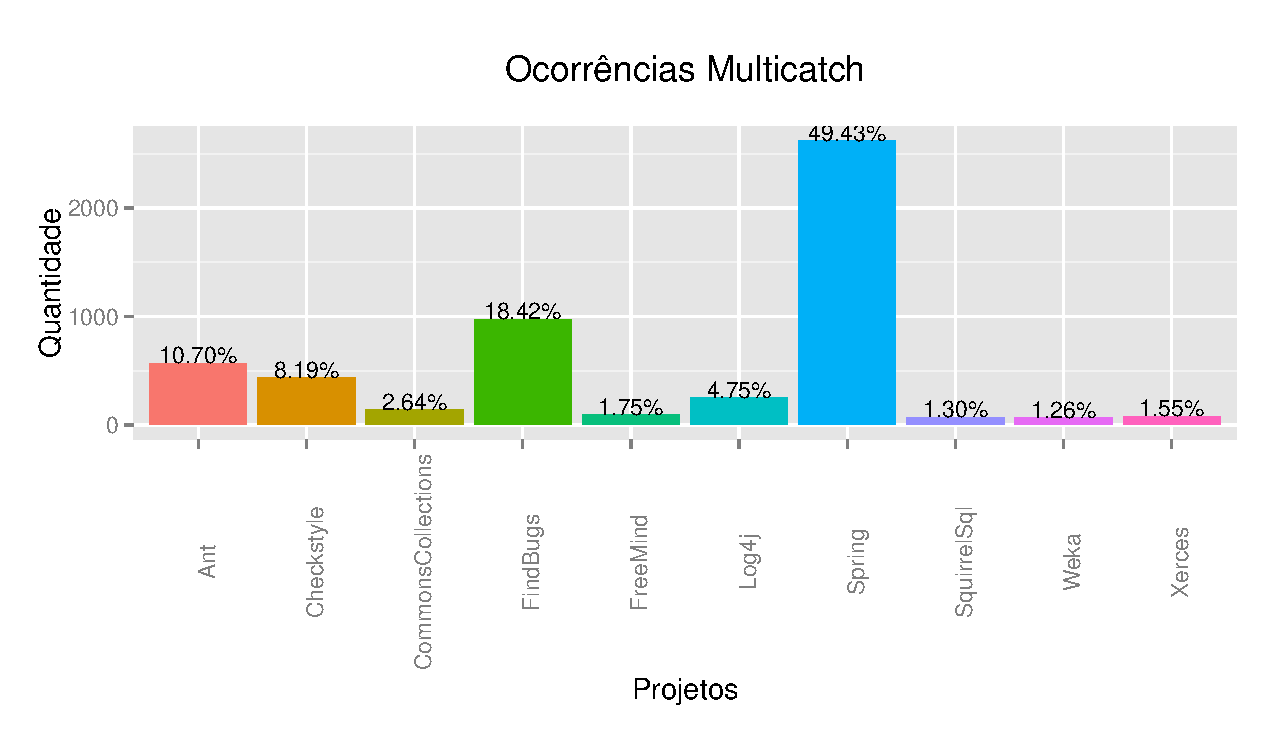
\includegraphics[width=13cm,height=7.8cm]{Imagens/ocorrenciasMulticatch}
	\label{fig:Muticatch}
	\caption{Oportunidades de \textit{Multicatch} nos projetos.}
\end{figure}
		

Considere os exemplos nas listagens {\color{red} X e Y}, 
encontrados na classe \texttt{AbstractNestablePropertyAccessor} do projeto \textit{Spring 4.2.0.RC2}. 
Neste caso, é possível reestruturar o c\'{o}digo para usar a constru\c c\~{a}o 
\texttt{multi-catch}, o que levaria a uma redu\c c\~{a}o de {\color{red} 40\%}  para 
esse trecho de código. Um simples \textit{refactoring} unindo todos os blocos 
que potencialmente se beneficiariam do uso de blocos \texttt{multi-catch} levaria a uma redução de 
68063 \acs{LOC}, tornando essa constru\c c\~{a}o  \'{u}til para reduzir a quantidade de 
linhas de c\'{o}digo em duplicidade de um projeto. 
\begin{lstlisting}[]
// Sem uso de Multicacth 17 LOC
try {...}
catch (ConverterNotFoundException ex) {
  PropertyChangeEvent pce = new PropertyChangeEvent(this.rootObject, this.nestedPath + propertyName, oldValue, newValue);
  throw new ConversionNotSupportedException(pce, td.getType(), ex);
}catch (ConversionException ex) {
  PropertyChangeEvent pce = new PropertyChangeEvent(this.rootObject, this.nestedPath + propertyName, oldValue, newValue);
  throw new TypeMismatchException(pce, requiredType, ex);
}catch (IllegalStateException ex) {
  PropertyChangeEvent pce = new PropertyChangeEvent(this.rootObject, this.nestedPath + propertyName, oldValue, newValue);
  throw new ConversionNotSupportedException(pce, requiredType, ex);
}catch (IllegalArgumentException ex) {
  PropertyChangeEvent pce = new PropertyChangeEvent(this.rootObject, this.nestedPath + propertyName, oldValue, newValue);
  throw new TypeMismatchException(pce, requiredType, ex);
}
\end{lstlisting}


\begin{lstlisting}
 //  Com uso de Multicatch 10 LOC
 try {...}
 catch (ConverterNotFoundException ex | IllegalStateException ex) {
   PropertyChangeEvent pce = new PropertyChangeEvent(this.rootObject, this.nestedPath + propertyName, oldValue, newValue);
   throw new ConversionNotSupportedException(pce, td.getType(), ex);
 }catch (ConversionException ex | IllegalArgumentException ex) {
   PropertyChangeEvent pce = new PropertyChangeEvent(this.rootObject, this.nestedPath + propertyName, oldValue, newValue);
   throw new TypeMismatchException(pce, requiredType, ex);
 }	
\end{lstlisting}

%Uma análise mais detalhada sobre \textit{JBoss, Spring, Hibernate e Findbugs} totalizando juntos 7778 ocorrências, iniciando na 3.0.0.M1 lançada em junho de 2009 até a mais recente até o momento 4.2.0.RC2. Para uma análise mais criteriosa será elaborada um detalhamento a partir da versão 4.0.0.M1 até a 4.2.0.RC2 totalizando 927 oportunidades de \textit{multicatch} 35\% das ocorrências no \textit{Spring}.\\

A figura: \ref{fig:ocorrenciasMulticatchVersoes} exibe as ocorrências nos projetos mais numerosos do estudo. Onde todas as ocorrências totalizam 17100 \acs{LOC} e após um simples \textit{refactoring}, 
conforme o exemplo anterior, obtem-se 5955 \acs{LOC} o que acarreta uma redução da ordem de 65\% de c\'{o}digo duplicado em blocos \texttt{catch}.

\begin{figure}[h]
	\center
	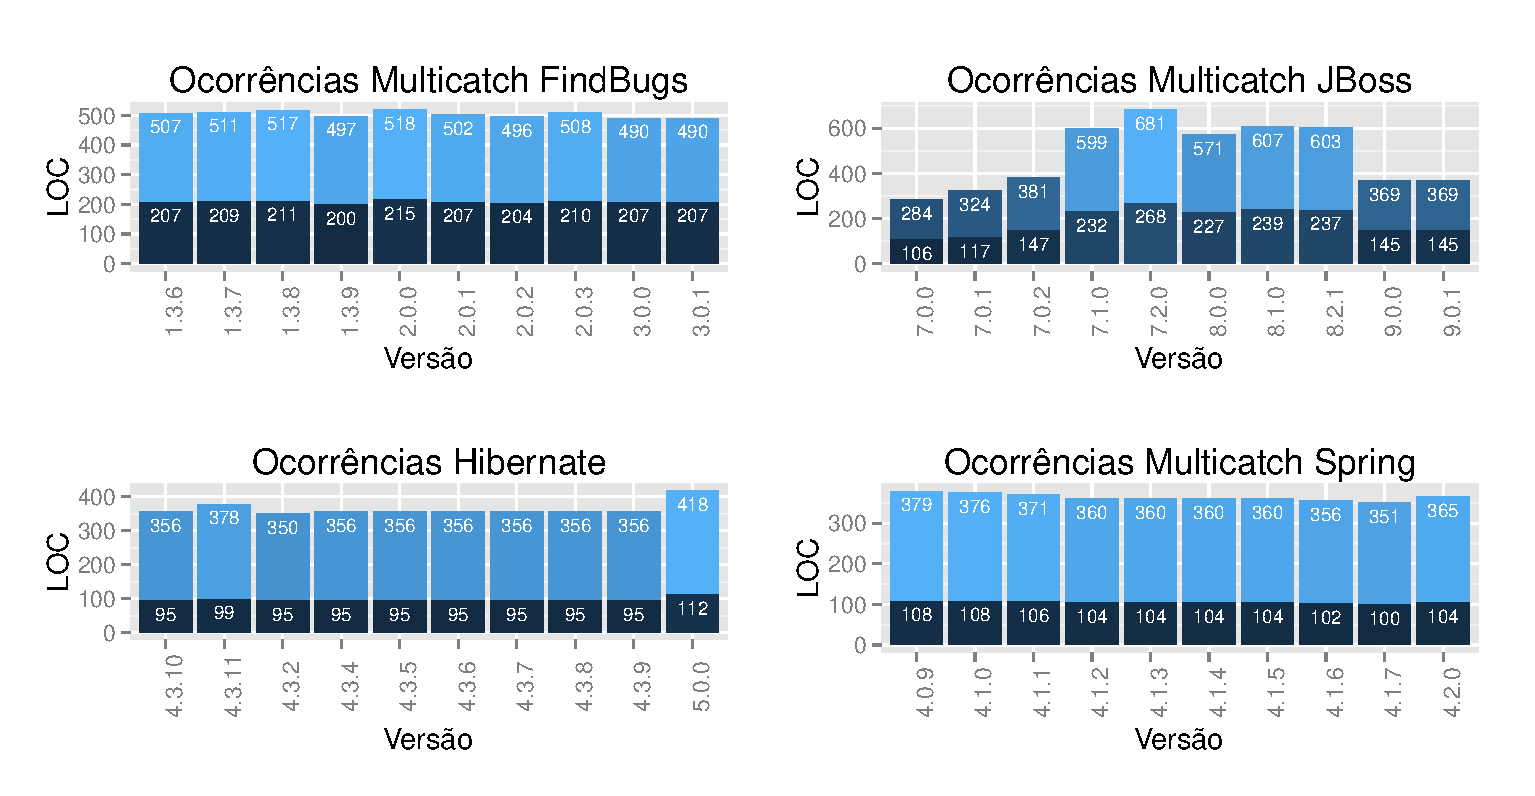
\includegraphics[height=8cm, keepaspectratio]{Imagens/ocorrenciasMulticatchVersoes}
	\label{fig:ocorrenciasMulticatchVersoes}
	\caption{Oportunidades de \textit{Multicatch} nos projetos.}
\end{figure}

